\documentclass[11pt,a4paper]{article}
\usepackage[margin=1in]{geometry}
\usepackage{hyperref}
\usepackage{enumitem}
\usepackage{graphicx}
\usepackage{xcolor}
\usepackage{longtable}

% -----------------------------------------------------
% bvraghav-tiet-ucs503p-article.sty
% -----------------------------------------------------

% Variable: Lab Instructor
\makeatletter \newcommand{\BvrSetLabInstructor}[1]{%
  \gdef\Bvr@LabInstructor{#1}}
% default
\newcommand{\Bvr@LabInstructor}{Dr. Raghav %
  B. Venkataramaiyer}
% public accessor
\newcommand{\BvrLabInstructorValue}{\Bvr@LabInstructor}
\makeatother

% Add subtitle
\usepackage{titling}
% -- Set title bold
\pretitle{\begin{center}\bfseries\fontsize{18bp}{18bp}\selectfont}
\makeatletter
\newcommand{\BvrSubtitle}[1]{%
  \posttitle{%
    \par\end{center}
    \begin{center}\large#1\end{center}
    \vskip 0.5em}%
}
\makeatother

% Hints in the section title(s)
\newcommand{\BvrHint}[1]{%
  {\normalfont\normalsize\itshape\hfill #1}}

% -----------------------------------------------------

\title{CreditSetu: A Dual-Path Credit Scoring \& Lending Marketplace for Microfinance}

\BvrSetLabInstructor{Dr. Raghav B. Venkataramaiyer}

\BvrSubtitle{%
  Prototype Stage Report for UCS503P  \\
  Submitted to: \BvrLabInstructorValue \\ \bfseries
  Thapar Institute of Engineering and Technology%
}

\author{
  Maanya Garg, CSED%
  \thanks{Roll No: \texttt{1024030564}}
  \and
  Kashvi Bansal, CSED%
  \thanks{Roll No: \texttt{1024030563}}
  \and
  Shreesh Gupta, CSED%
  \thanks{Roll No: \texttt{1024030565}}
  \and
  Shivam Raj, CSED%
  \thanks{Roll No: \texttt{1024031140}}
}

\date{\today}

\begin{document}
\maketitle

\begin{abstract}
CreditSetu is a dual-path credit-scoring and lending-marketplace
platform for microfinance in India. Its core proposition is that every
borrower builds their \emph{own} credit score from their own repayment
history, while a borrower who belongs to a Self-Help Group (SHG) gets a
trust-based bootstrap head start from their group's track record and an
independent borrower starts from a flat base and builds purely from
scratch. Scores are produced by an XGBoost classifier and explained
feature-by-feature with SHAP, so a borrower or lender sees not just a
number but why it is what it is. Lenders formally partner with specific
SHGs through an approve/reject linkage rather than open lending to
anyone, and a loan marketplace lets lenders make offers and borrowers
request loans directly. At the prototype stage, the system has been
rebuilt around four separate, role-gated logins (Borrower, Lender, SHG,
Admin), each authorized server-side and scoped strictly to that role's
own data, and extended with a live borrower repayment flow (a wallet
balance and a dummy payment gateway) so a borrower's actions -- not
just offline synthetic history -- move their own score. This report
covers the system's architecture, data model, scoring methodology,
feasibility, what has actually been built and verified working, and
the accompanying UML design diagrams.
\end{abstract}

\textbf{Keywords:} Microfinance, Credit Scoring, XGBoost, SHAP,
Explainable AI, Self-Help Groups, Role-Based Access Control, FastAPI,
React.

\section{Introduction%
\BvrHint{\ldots background and motivation}}

Microfinance lending in India serves two kinds of borrowers very
unevenly. A member of a Self-Help Group (SHG) benefits from the
group's collective track record and social accountability, while an
independent borrower with no group affiliation and no prior loan has
nothing a lender can score against -- the classic cold-start problem.
Where informal scoring does exist, it is rarely explainable: a
borrower or lender sees a number with no account of \emph{why} it is
what it is, which undermines both borrower trust and lender diligence.
Structured, auditable relationships between a specific lender and a
specific SHG are also usually absent -- a lender either serves an
entire group's members or none of them, with no formal, revocable
agreement in between.

An earlier version of this project (\texttt{Sahara MFI}, a
Node/Express + MySQL application) addressed SHG-only scoring through a
hand-written SQL formula, with no independent-borrower path, no
machine-learning component, and no lender marketplace. CreditSetu is a
from-scratch rebuild: the general domain (SHGs, loans, repayments,
credit scores) carries over, but the schema, scoring approach, and
system design are new, driven by the dual-path requirement that did
not fit the old single-path schema.

\subsection{Problem Statement}
\begin{itemize}[leftmargin=0.7cm]
    \item \textbf{Cold-start scoring:} an independent borrower with no
    formal credit history cannot be scored by a model trained only on
    borrowers who already have repayment history.
    \item \textbf{Opaque scoring:} even where a score exists, it is
    rarely explained in a way a borrower or lender can act on.
    \item \textbf{No formal SHG-lender relationship:} lending decisions
    at group level are informal and unauditable.
    \item \textbf{Undifferentiated access:} in an open system, a
    borrower, a lender, and an SHG all see the same data, with no
    role-appropriate, access-controlled view for any of them.
\end{itemize}

\subsection{Objectives}
\begin{itemize}[leftmargin=0.7cm]
    \item Build a dual-path scoring engine that gives SHG members a
    fair, group-earned head start while letting independent borrowers
    build a score purely from their own behaviour.
    \item Make every score explainable, feature by feature, using
    SHAP.
    \item Formalize the SHG-lender relationship as an explicit
    approve/reject linkage.
    \item Separate the system into four role-gated views (Borrower,
    Lender, SHG, Admin), each authorized server-side, so no role can
    see another's data.
    \item Let a borrower's own actions -- not just offline synthetic
    history -- move their own score, via a live repayment flow.
\end{itemize}

\section{Related Work%
\BvrHint{\ldots existing approaches}}

Traditional microfinance credit assessment relies heavily on group
liability and manual field-agent judgement, with limited use of
statistical or machine-learning scoring. Where formal credit bureaus
exist (e.g. CIBIL in India), they score individuals with an existing
formal credit history and have no mechanism for a first-time,
group-affiliated borrower to inherit a trust signal from their group.
Commercial microfinance information systems (including the team's own
earlier \texttt{Sahara MFI} build) typically implement a single,
SHG-only scoring formula with no cold-start path for independent
borrowers and no per-feature explanation of the resulting score.
Explainable-AI techniques such as SHAP \cite{shap} have seen adoption
in consumer credit scoring in developed markets, but are less common
in microfinance-specific tooling, where model opacity and the
cold-start problem are usually treated as separate, unrelated
concerns rather than solved together through an explicit bootstrap-to-
model blend, as CreditSetu does.

\section{Proposed Methodology%
\BvrHint{\ldots system design}}

\subsection{System Architecture}
CreditSetu is a 3-tier web application:
\begin{itemize}[leftmargin=0.7cm]
    \item \textbf{Frontend:} a React (Vite) single-page application
    with four role-gated dashboards (Borrower, Lender, SHG, Admin) and
    a public landing page, styled as a government-portal-style
    demonstration platform (clearly labelled as such, not
    impersonating any real government property).
    \item \textbf{Backend API:} FastAPI, exposing REST endpoints under
    \texttt{/api}, with bearer-token session authentication per role
    and server-side authorization scoping every query to the
    authenticated caller's own identity.
    \item \textbf{Database:} SQLAlchemy over SQLite for the
    demonstration deployment (a one-line \texttt{DATABASE\_URL}
    environment-variable change moves this to Postgres for concurrent
    production use, with no code changes).
    \item \textbf{ML pipeline:} offline scripts (not imported by the
    API at request time) for synthetic data generation, model
    training, and batch scoring, producing artifacts the API serves.
\end{itemize}

\subsection{Data Model}
The schema has thirteen core tables plus the role-based-access and
payments additions made during this iteration: \texttt{districts},
\texttt{shgs}, \texttt{individuals} (the dual-path pivot --
\texttt{shg\_id} is nullable, and NULL means independent), plus
per-role \texttt{...\_sessions} tables (individual, lender, shg,
admin), \texttt{shg\_attendance\_records}, \texttt{savings\_records},
\texttt{lenders}, \texttt{shg\_lender\_links} (the approve/reject
table, extended with an \texttt{initiated\_by\_role} column so the UI
can correctly determine which side may approve/reject a given link),
\texttt{loans} (extended with a borrower-chosen
\texttt{target\_lender\_id} on the request side), \texttt{repayment\_events},
\texttt{credit\_scores} (append-only score history, not a single
mutable column), \texttt{score\_explanations} (per-feature SHAP
contribution, in score points, per score), \texttt{loan\_offers} and
\texttt{loan\_requests} (the two-directional marketplace flow), and
\texttt{anomaly\_flags}. The full class-level detail of every table,
field, and relationship is given in the Class Diagram in
Section~\ref{sec:class-diagram}.

\subsection{Scoring Algorithm}
\textbf{Input:}
\begin{itemize}[leftmargin=0.7cm]
    \item An individual's loans, repayment events, savings records,
    and (if SHG-linked) attendance records.
    \item Trained XGBoost classifier and its SHAP
    \texttt{TreeExplainer}.
    \item Configured bootstrap parameters: \texttt{SCORE\_MIN},
    \texttt{SCORE\_MAX}, \texttt{INDEPENDENT\_BASE\_SCORE}, the SHG
    peer-trust bootstrap formula, and \texttt{HISTORY\_MATURITY\_EVENTS}.
\end{itemize}
\textbf{Output:} a score in $[\texttt{SCORE\_MIN}, \texttt{SCORE\_MAX}]$,
a risk category, the scoring basis (\texttt{shg\_bootstrap} /
\texttt{independent\_bootstrap} / \texttt{model}), and a per-feature
SHAP explanation summing to \texttt{score - SCORE\_MIN}.
\begin{enumerate}[leftmargin=0.7cm]
    \item Turn the individual's raw history into $\sim$16 engineered
    features (repayment rate, savings regularity, SHG tenure, peer
    repayment rate, etc.); a missing input is represented as NaN, never
    silently zeroed.
    \item Count \texttt{n\_repayment\_events} for this individual.
    \item If zero: return the pure prior -- the SHG bootstrap (derived
    from the group's own aggregate repayment/attendance rate) for an
    SHG-linked individual, or the flat \texttt{INDEPENDENT\_BASE\_SCORE}
    for an independent one. No model call.
    \item If between 1 and \texttt{HISTORY\_MATURITY\_EVENTS}: linearly
    blend the prior and the trained model's prediction, weighted by how
    much real history has accumulated.
    \item If at or past \texttt{HISTORY\_MATURITY\_EVENTS}: use the
    model's prediction alone.
    \item Run the SHAP \texttt{TreeExplainer} on the model's output
    (or, for a pure-prior score, synthesize an explanation anchored on
    the model's own baseline prediction rather than the floor, so a
    high-risk borrower's explanation does not collapse to
    near-empty -- see Section~\ref{sec:bugs}).
    \item Persist the score as a new, append-only \texttt{CreditScore}
    row and its \texttt{ScoreExplanation} rows.
\end{enumerate}

\subsection{Role-Based Access Control}
Four roles -- Borrower, Lender, SHG, Admin -- each log in separately
(phone+password for borrowers, username+password for the other three,
all demo-seeded with the same hashing scheme, no JWT). Every endpoint
in the API requires the correct role's bearer token and derives "my
own data" from the session, never from a client-supplied id; an
out-of-scope request is rejected with 401 (no/bad token) or 403 (wrong
role or wrong identity), enforced server-side rather than only hidden
in the UI. Table~\ref{tab:access-matrix} summarises what each role may
see.

\begin{table}[h]
\centering
\begin{tabular}{|l|l|}
\hline
\textbf{Role} & \textbf{Sees} \\
\hline
Borrower & Own score/history/SHAP explanation/improvement tips, \\
         & own SHG's public stats, own loans, own requests/offers, \\
         & the full lender directory (read-only). \\
\hline
Lender & SHGs browsable by district, member lists for SHGs they \\
       & are linked to, incoming loan requests, own reputation score. \\
\hline
SHG & Own members and stats, own linked/pending lender links. \\
\hline
Admin & Read-only, platform-wide: all borrowers/SHGs/lenders, \\
      & district stats, anomaly flags, model health. \\
\hline
\end{tabular}
\caption{Role $\to$ data-access matrix}
\label{tab:access-matrix}
\end{table}

\subsection{Repayment and Payment Gateway}
A borrower can direct a loan request at a specific eligible lender (in
addition to the existing broadcast-to-all-eligible-lenders behaviour),
with a retarget option if a targeted request is declined. Once a loan
is active, "amount due this cycle" is derived from the count of
existing repayment events on that loan (not from elapsed calendar
time), so a loan is payable the instant it is disbursed rather than
only after a real due date has passed -- necessary for the feature to
be usable by a live user rather than only replayable against backdated
data. A dummy payment gateway (clearly labelled as non-real) shows the
borrower's wallet balance and the amount due per active loan; if the
wallet cannot cover the borrower's \emph{total} dues across all active
loans this cycle, payment of every loan is blocked, not just the one
clicked. A successful payment creates a real \texttt{RepaymentEvent},
updates the loan's outstanding balance and status, and recomputes the
credit score in the same transaction.

\section{Feasibility Report%
\BvrHint{\ldots can this actually be built and run}}

\subsection{Technical Feasibility}
Every component uses mature, well-documented open-source tooling
already proven at this scale: FastAPI and SQLAlchemy for the API and
ORM, XGBoost and SHAP for scoring and explanation, scikit-learn for
k-means district clustering and isolation-forest anomaly detection,
and React/Vite for the frontend. No component requires novel research
or unavailable infrastructure. The team has already built, run, and
fixed real defects in this stack (see Section~\ref{sec:bugs}),
demonstrating the architecture is technically sound in practice, not
just on paper.

\subsection{Operational Feasibility}
The system runs on a single machine for demonstration (SQLite,
\texttt{uvicorn --reload}, \texttt{npm run dev}) with no external paid
service dependency. A production deployment would swap SQLite for a
managed Postgres instance via a single environment variable and add a
proper secrets/password-hashing setup in place of the deliberately
minimal demo scheme -- both are additive changes, not architectural
rewrites.

\subsection{Economic Feasibility}
All tooling used is free and open-source; there is no licensing cost.
The only cost at production scale would be standard cloud hosting
(a database instance and a small API/web server), which is
proportionate to any comparable small-to-medium SaaS deployment and
not a blocker for a course project or an early pilot.

\subsection{Schedule Feasibility}
The 8-stage plan (synthetic data generation, scoring engine,
cold-start bootstrap, SHG-lender linkage, lender matching/offers,
frontend, geo-clustering, anomaly detection) was completed and
verified end-to-end before this iteration began. The current
iteration -- role separation, server-side authorization, targeted
requests, and the live repayment flow -- was completed, tested against
the live API and browser, and is documented with real before/after
verification (Section~\ref{sec:results}), indicating the remaining
course milestones (further hardening, the Final Report) are reachable
within the semester timeline.

\section{Implementation and Results%
\BvrHint{\ldots what actually works, verified}}
\label{sec:results}

All figures in this section are measured against the live system, not
estimated.

\subsection{Current Scale}
The seeded dataset spans 1{,}079 individuals (659 SHG-linked, 420
independent), 51 SHGs, 6 lenders, and 10 districts, with over 1{,}600
loans and their associated repayment events.

\subsection{Verified End-to-End: Loan Lifecycle and Score Impact}
A real borrower account was taken through the full live flow with no
manual database edits: request a loan $\to$ have it approved by a real
lender login $\to$ repay it through the payment gateway. The credit
score moved from 596 (Medium risk) to 886 (Very Low risk) as real
on-time repayment history crossed \texttt{HISTORY\_MATURITY\_EVENTS},
with the scoring basis switching from \texttt{independent\_bootstrap}
to \texttt{model} -- exactly the behaviour the methodology in
Section~3.3 specifies.

\subsection{Verified: Access Control}
Cross-role and cross-identity requests were tested directly against
the live API (e.g. a borrower token fetching another borrower's
record, a lender token fetching an SHG it is not linked to) and
correctly rejected with 401/403 in every case tested.

\subsection{Bugs Found and Fixed}
\label{sec:bugs}
Several real defects were found by running the system end-to-end
(training on real data, hitting the live API, and exercising the live
frontend) rather than by reading the code:
\begin{enumerate}[leftmargin=0.7cm]
    \item A hard \texttt{missed\_fraction > 0.4} cliff made the
    synthetic default label a near coin-flip at the boundary --
    replaced with a smooth, probabilistic default rule.
    \item SHAP explanations were allocated as a share of
    \texttt{score - floor}, which silently went nearly blank for
    borrowers scoring near the floor -- exactly the people who most
    need an explanation. Fixed by anchoring on the model's own baseline
    prediction instead.
    \item An SHG-lender link's \texttt{requested\_date} could land in
    the future for a recently formed SHG -- capped at today.
    \item k-means cluster labels were inverted (worst cluster labelled
    "High Trust").
    \item Missing indexes on every foreign key, and missing
    \texttt{\_\_init\_\_.py} files in three subpackages.
    \item An unbounded eligible-borrowers table rendered 351 rows with
    no cap -- capped at 25 with a "showing top N of M" note.
    \item A frontend/backend pagination mismatch made roughly half the
    population unreachable by search -- replaced with real server-side
    search.
    \item The "Approve/Reject Partnership" buttons on the Lender and
    Admin dashboards referenced a field name (\texttt{link\_id}) that
    does not exist in the API response (the real field is \texttt{id})
    -- every click silently called the decide endpoint with
    \texttt{undefined}, meaning a lender could never actually approve
    or reject an SHG link through the UI. Fixed and verified live.
    \item \texttt{GET /api/shgs} computed each SHG's aggregate
    repayment/attendance rate as a Python property walking
    \texttt{members -> loans -> repayment\_events} per SHG -- an N+1
    pattern materializing on the order of 25{,}000+ ORM objects per
    request against the real dataset, measured at 1{,}101--1{,}322\,ms
    median. Replaced with three \texttt{GROUP BY} SQL aggregates:
    14.5--26.7\,ms median, a $\sim$75$\times$ improvement, with
    identical response content verified before and after.
\end{enumerate}

\section{Conclusion and Future Scope%
\BvrHint{\ldots where this stands and what's next}}

At the prototype stage, CreditSetu has a working, explainable,
dual-path scoring engine; a formal SHG-lender linkage; a two-directional
loan marketplace with targeted requests; four separately authorized
role-based views with server-side access control; and a live borrower
repayment flow whose impact on credit score has been verified against
a real account, not just claimed. Real defects, including one that
silently broke a core lender action and one with a measured
75$\times$ performance impact, were found and fixed by exercising the
live system rather than only reading the code.

Remaining work toward the Final Report: periodic re-scoring so genuine
score-history trends accumulate over time (currently limited by how
few times the batch-scoring pipeline has actually been run); admin
account-management/moderation actions beyond the current read-only
oversight view; and replacing the deliberately minimal demo
bearer-token/password scheme with production-grade hashing and
short-lived signed tokens. The independent-vs-SHG base-score gap
remains a stated policy parameter rather than something the data
derived, and is flagged as a candidate for a fairness sensitivity
analysis in the Final Report.

\bibliographystyle{plain}
\begin{thebibliography}{9}
\bibitem{shap}
Lundberg, S. M., \& Lee, S.-I. (2017). A Unified Approach to
Interpreting Model Predictions. \textit{Advances in Neural Information
Processing Systems (NeurIPS)}.
\bibitem{xgboost}
Chen, T., \& Guestrin, C. (2016). XGBoost: A Scalable Tree Boosting
System. \textit{Proceedings of the 22nd ACM SIGKDD International
Conference on Knowledge Discovery and Data Mining}.
\end{thebibliography}

\newpage
\appendix
\section{Use Case Diagram}
\label{sec:usecase-diagram}
Four actors (Borrower, Lender, SHG, Admin) against every real use case
grounded in the actual API routers and dashboards. Full written
use-case scenarios (preconditions, main/alternate flows,
postconditions) for the six most important use cases are in
\texttt{docs/uml/use-case-diagram.md} in the repository, alongside the
PlantUML source (regenerate/edit at
\url{https://www.plantuml.com/plantuml/}).

\begin{figure}[h]
\centering
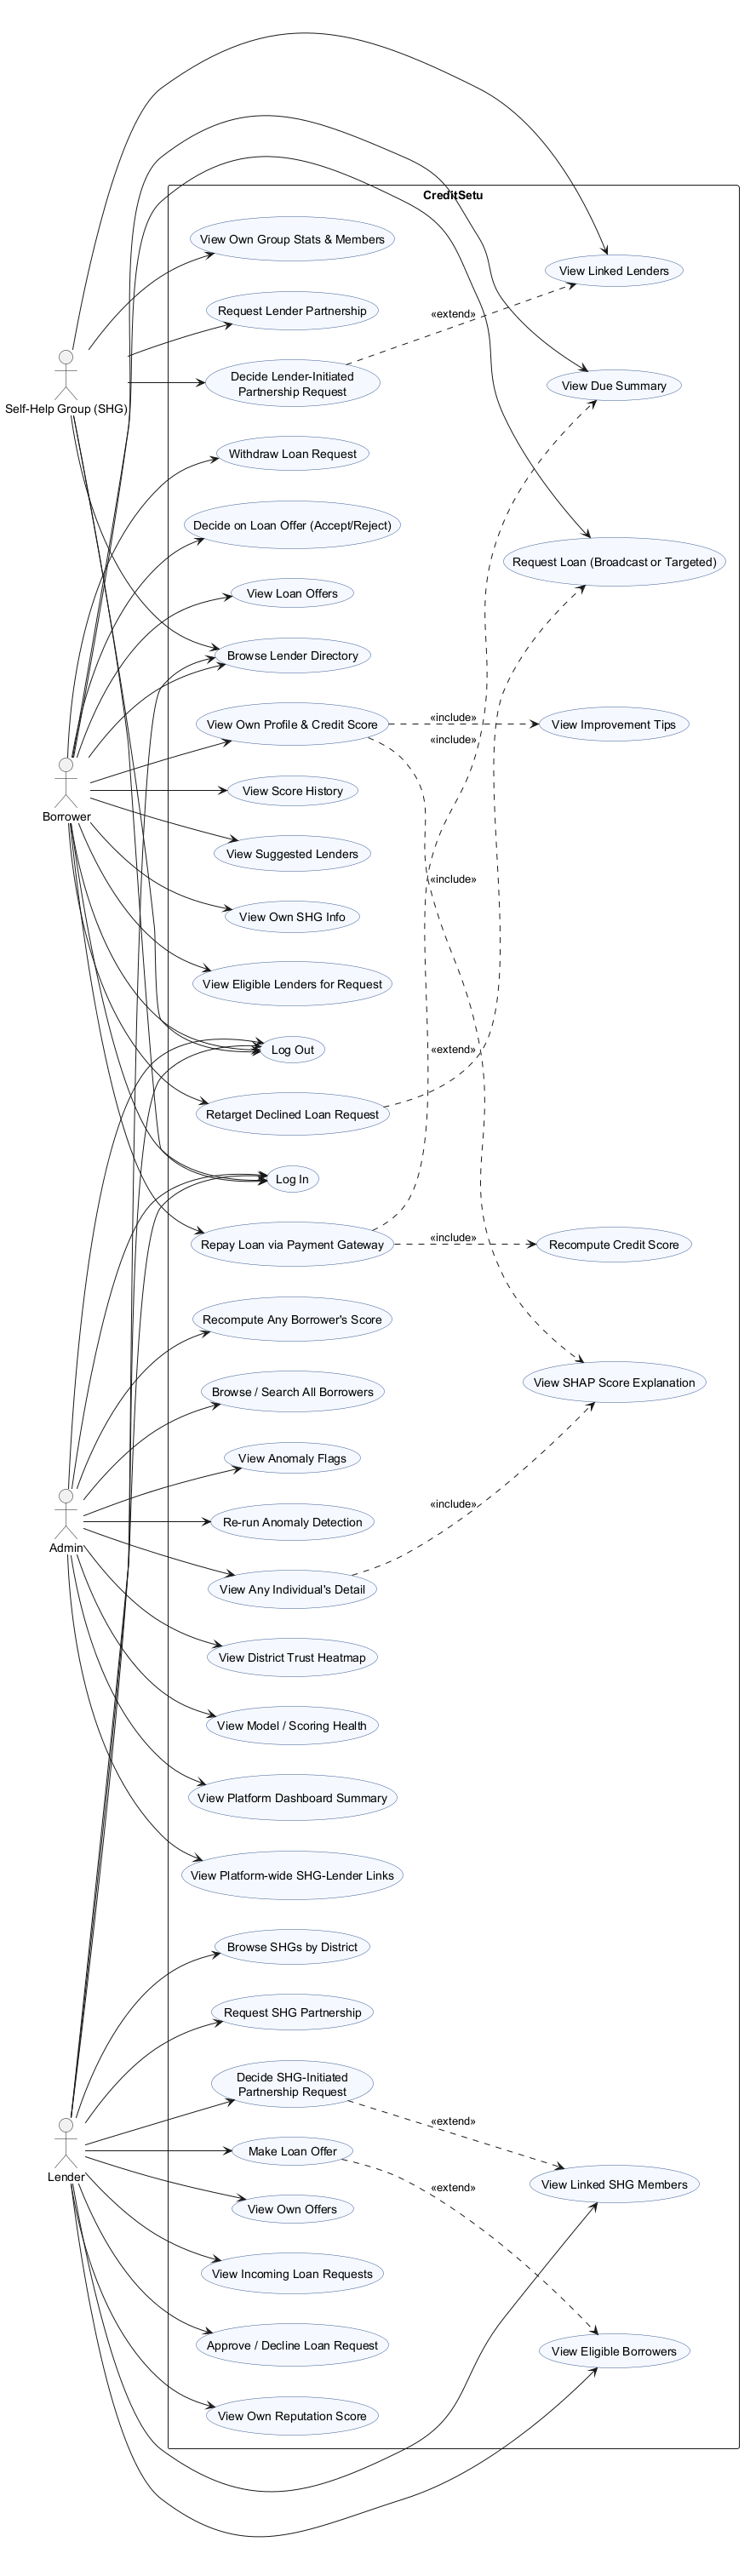
\includegraphics[height=0.85\textheight]{figures/use-case-diagram.png}
\caption{CreditSetu use case diagram}
\end{figure}

\clearpage
\section{Class Diagram}
\label{sec:class-diagram}
The real SQLAlchemy schema (\texttt{app/models.py}), including the
role-based-access session tables and the payments-feature additions.
See \texttt{docs/uml/class-diagram.md} for the PlantUML source and the
accompanying design-decision notes (the nullable \texttt{shg\_id}
dual-path pivot, append-only \texttt{CreditScore} history, and the
\texttt{SHGLenderLink} many-to-many approve/reject table).

\begin{figure}[h]
\centering
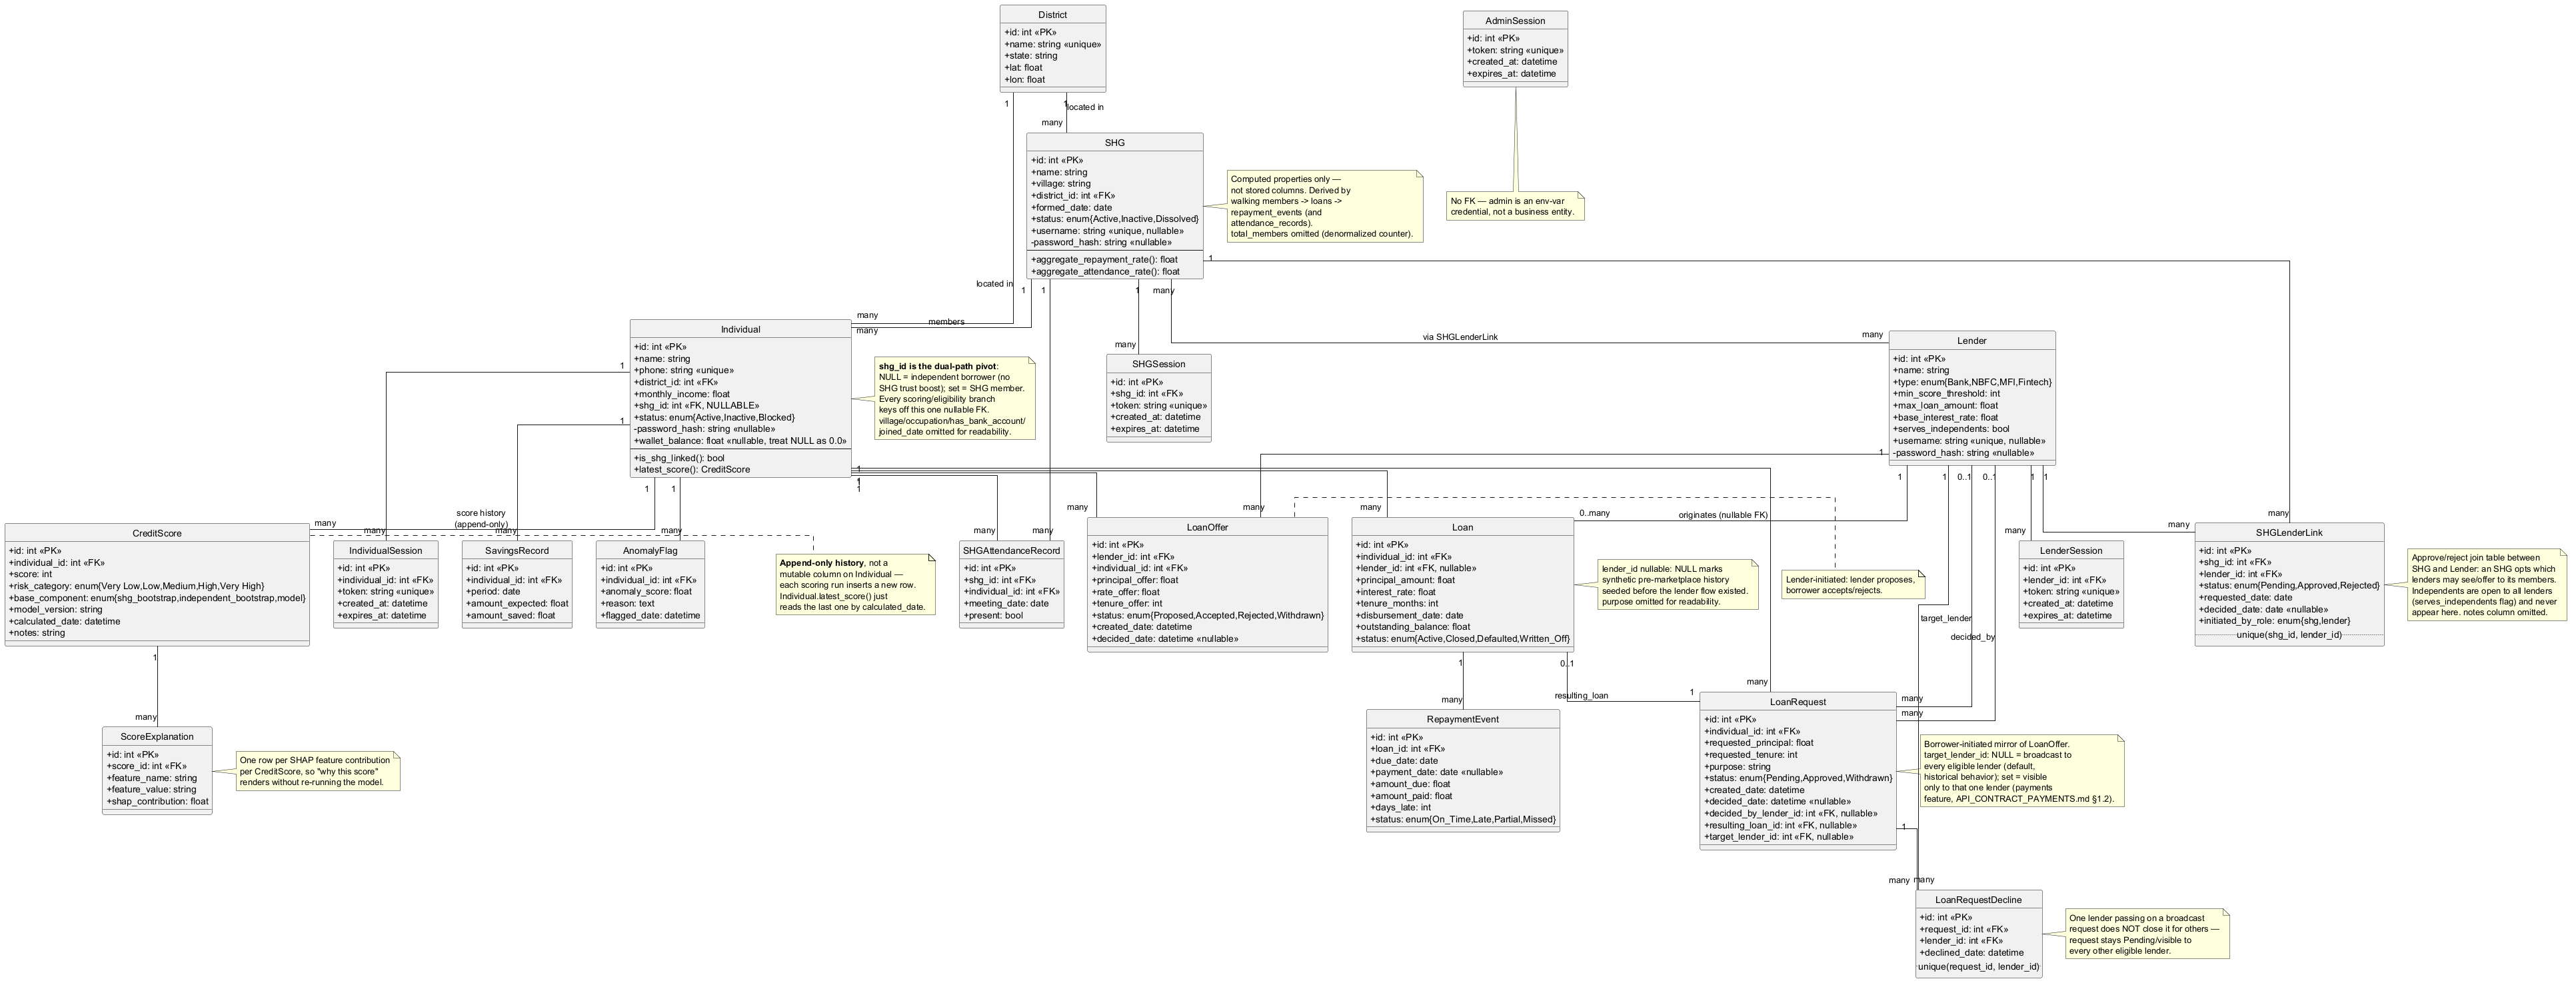
\includegraphics[width=\textwidth]{figures/class-diagram.png}
\caption{CreditSetu class diagram}
\end{figure}

\clearpage
\section{Activity Diagram}
\label{sec:activity-diagram}
The real request $\to$ approval $\to$ repayment $\to$ rescoring
control flow, with Borrower / System (Backend) / Lender swimlanes,
including the aggregate insufficient-funds gate and the race-condition
guard on the wallet balance. See \texttt{docs/uml/activity-diagram.md}
for the PlantUML source and a step-by-step prose walkthrough mapping
each step to the real backend function it corresponds to.

\begin{figure}[h]
\centering
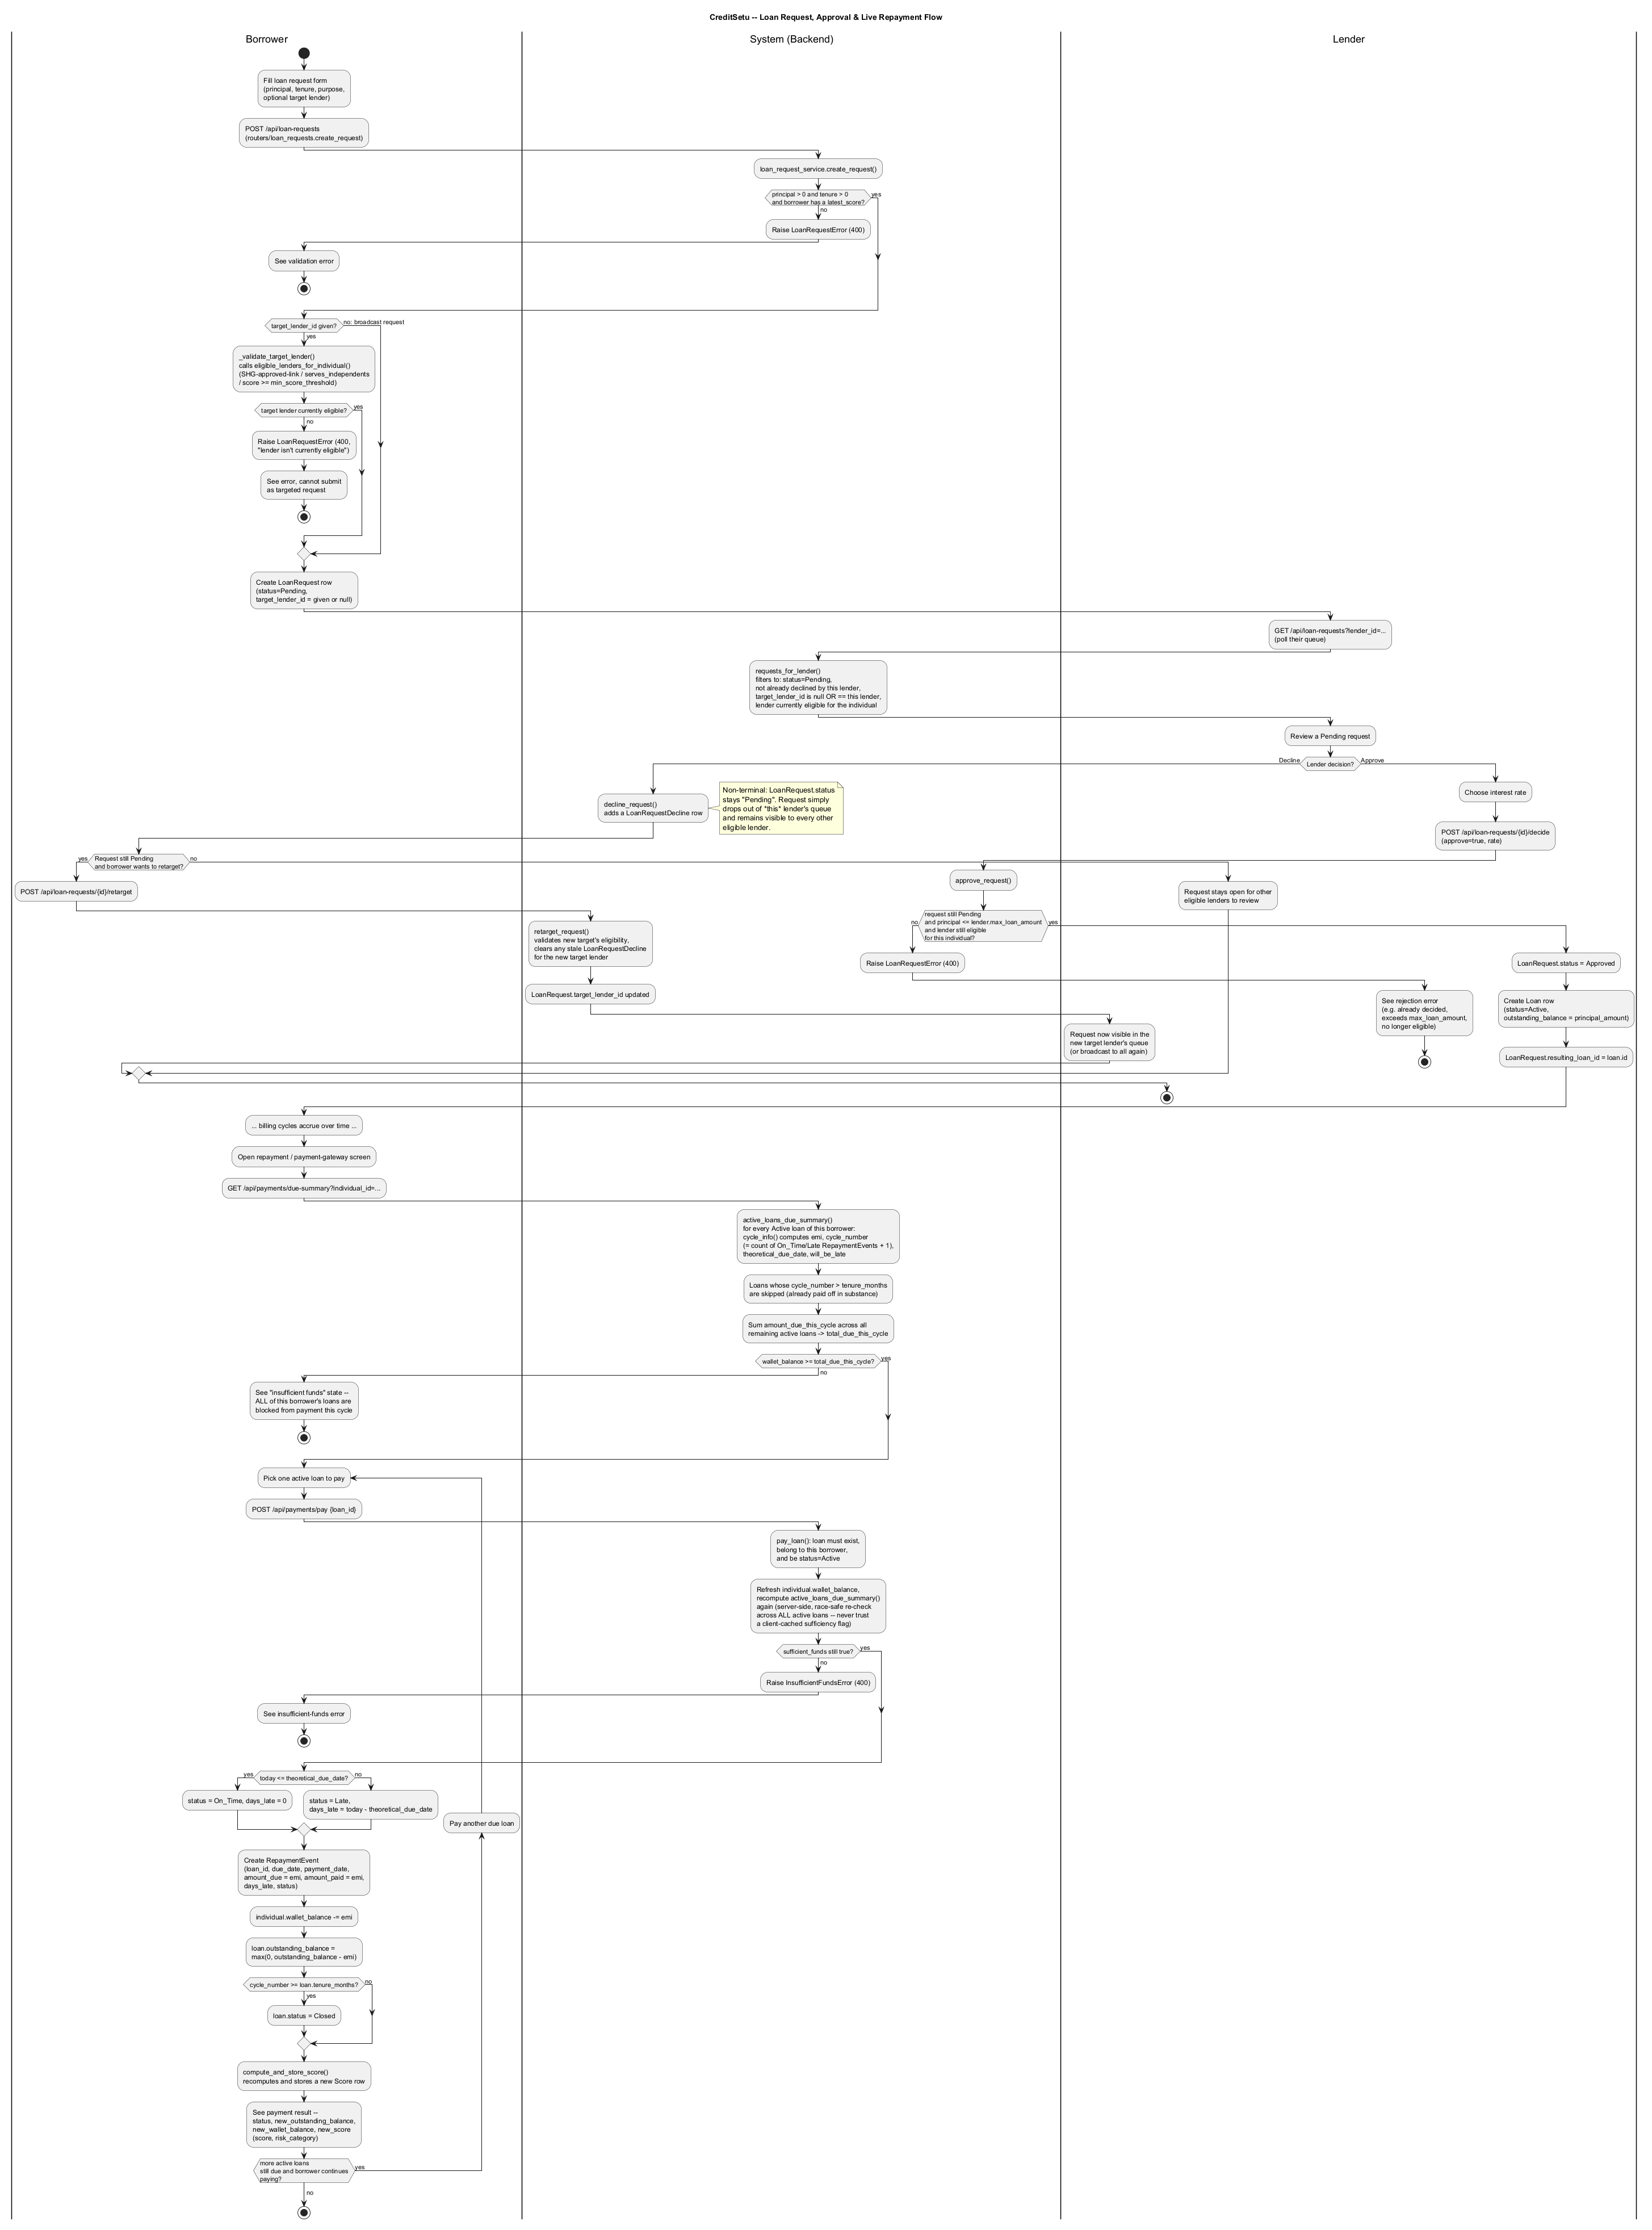
\includegraphics[height=0.85\textheight]{figures/activity-diagram.png}
\caption{CreditSetu activity diagram: loan request, approval, and live repayment}
\end{figure}

\end{document}
